\documentclass[a4paper]{article}
\usepackage{longtable}
\usepackage{graphicx}
\usepackage{hyperref}
\usepackage{amsmath, amssymb}
\usepackage[italian]{babel}
\usepackage[T1]{fontenc}
\usepackage[utf8]{inputenc}
\usepackage[a4paper, margin=0.75in]{geometry}
\usepackage{quoting}
\usepackage{listings}
\usepackage{verbatim}
\usepackage[section]{placeins}


\hypersetup{
    hidelinks
}


\title{Progetto Big Data e Business Intelligence}
\author{Ollari Ischimji Dmitri}


\begin{document}

    \begin{titlepage}
        \maketitle
    \end{titlepage}

    \tableofcontents
    

    \begin{abstract}
        In questo documento verrano descritti i ragionamenti, le tecniche e gli strumenti utilizzati per 
        cercare di ottenere il miglior risultato possibile nel task di classificazione multi classe sul dataset heart disease.
    \end{abstract}

    \section{Look at the bigger pictures}


    Questo dataset proviene dal \textbf{\href{https://archive.ics.uci.edu/ml/datasets/heart+disease}{UCI Machine Learning Repository}},
    viene utilizzato per task di classificazione supervisionate multiclasse poichè presenta
    76 features, di cui una viene usata come target.

    Lo scopo di questa task di classificazione è quello di poter distinguere le 5 classi del dataset:
    \begin{enumerate}
        \item Sano
        \item Malato 1
        \item Malato 2
        \item Malato 3
        \item Malato 4
    \end{enumerate}

    Dove i vari malati si suddividono in classi (dalla 1 alla 4) in funzione della gravità.

    Per valutare l'accuratezza del modello utilizzato, essendo un dataset sbilanciato, verranno utilizzate:
    \begin{itemize}
        \item Precision
        \item Recall
        \item F-1 Score
    \end{itemize}


    Considerando la tipoliga di task, sarebbe preferibile aver il minor numero di falsi positivi possibili.

    Nel peggiore dei casi sarebbe preferibile sarebbe preferibile mantenere un recall più alto a discapito del precision score.

    \section{Get the data}
    
    \begin{center}
        \scalebox{0.8}{
        \def\arraystretch{1.5}
            \begin{tabular}{| p{20mm} | c | p{100mm} |}
            \hline
            Features Numero & Nome & Descrizione \\
            \hline
            1 & ID & Identificativo del paziente \\
            2 & CCF & Social Securty Number \\
            3 & AGE & Età \\
            4 & SEX & Sesso del paziente (1 = M, 0 = F) \\
            5 & PAINLOC & Posizione del dolore toracico (1 = substernal, 0 = altro) \\
            6 & PAINEXER & dolore al petto provocato da sforzo = 1, altro = 0 \\
            7 & RELREST & dolore passato dopo il riposo = 1, no = 0 \\
            8 & PNCADEN & summa di 5,6 e 7 \\
            9 & CP & Tipologia di dolore al petto: 
            \small{
                \begin{itemize}
                    \item tipica angina(malattia cardiaca) = 1
                    \item angina atipica = 2
                    \item non angina = 3
                    \item asintomatico = 4
                \end{itemize}} \\
            10 & TRESTBPS & Pressione a riposo \\
            11 & HTN & storia di ipertensione 1 = si, 0 = no \\
            12 & CHOL & colesterolo \\
            13 & SMOKE & 1 = fumatore, 0 = non fumatore \\
            14 & CIGS & sigarette al giorno \\
            15 & YEARS & anni di fumo \\
            16 &  FBS & zuccheri nel sangue a digiuno maggiori di $120mg/dl$, 1 = vero, 0 = falso \\
            17 & DM & Storia di diabete 1 = si, 0 = no \\
            18 & FAMHIST & presenza in famiglia di patologie alle coronarie \\
            19 & RESTECG & Elettrocardiogramma a riposo, 0 = normale, 1 = anormale \\
            20 & EKGMO & Mese della lettura per ECG \\
            21 & EKGDAY & Giorno della lettura per ECG \\
            22 & EKGYR & Anno della lettura per ECG \\
            23 & DIG & Usato il "digitalis" durante ECG? 1 = si, 0 = no \\
            24 & PROP & Beta Blocker usato durante ECG, 1 = si, 0 = no \\
            25 & NITR & nitrato usato nell'ECG, 1 = si, 0 = no \\
            26 & PRO & Calcio bloccato nelle letture dell'ECG, 1 = si, 0 = no \\
            27 & DIURETIC & usato un diuretico, 1 = si, 0 = no \\
            28 & PROTO & Protocollo usato per l'esercizio(classe da 1 a 12) \\
            29 & THALDUR & durata esercizio in minuti \\
            30 & THALTIME & Tempo dove è stata rilevata una depressione \\
            31 & MET & metriche raggiunte \\
            32 & THALACH & Battiti masimi \\
            33 & TAHLREST & Battiti cuore a riposo \\
            34 & TPEAKBPS & Picco di pressione durante l'esercizio (parte 1) \\
            35 & TPEAKBPD & Picco di pressione durante l'esercizio (parte 2) \\
            36 & DUMMY & dummy \\
            37 & TRESTBPD & pressione a riposo \\
            38 & EXANG & Angina indotta dall'esercizio? 1 = si, 0 = no \\
            39 & XHYPO & Calo di pressione indotto dall'esercizio? 1 = si, 0 = no \\
            40 & OLDPEAK & calo di pressione indotto a riposo \\
        \end{tabular}
    }
    
    \scalebox{0.8}{
        \def\arraystretch{1.5}
        \begin{tabular}{| p{20mm} | c | p{100mm} |}
            \hline
            Features Numero & Nome & Descrizione \\
            \hline
            
            41 & SLOPE & inclinazioen(?!) del picco sotto esercizio:
            \small{\begin{itemize}
                \item 1 = upsloping
                \item 2 = flat
                \item 3 = downsloping
            \end{itemize}} \\
            42 & RLDV5 & massima a riposo \\
            43 & RLDV5E & massima in sforzo \\
            44 & CA & Numero di vasi maggiori colorati dalla fluoroscopia \\
            45 & RESTCKM & Irrilevante?! \\
            46 & EXERCKM & Irrilevante?! \\
            47 & RESTEF & non capisco \\
            48 & RESTWM & Movimento a riposo anormale(classi da 0 a 3) \\
            49 & EXEREF & espulsione frazionata radionucolide dovuta a sforzo \\
            50 & EXERWM & Non capisco \\
            51 & THAL & scansione al "taglium" durante l'esercizio:
            \small{\begin{itemize}
                \item 3 = normale
                \item 6 = difetto fisso
                \item 7 = difetto reversibile
            \end{itemize}} \\
            52 & THALSEV & non usata \\
            53 & THALPUL & non usata \\
            54 & EARLPUL & non usata \\
            55 & CMO & mese della cateterizzazione cardiaca?! \\
            56 & CDAY & giorno della cateterizzazione cardiaca?! \\
            57 & CYR & anno della cateterizzazione cardiaca?! \\
            58 & NUM & Rappresenta la classe che identifica la presenza e lo stato della malattia(usato come Y) \\
            59 & LMT &  \\
            60 & LADPROX & \\
            61 & LADDIST & \\
            62 & DIAG & \\
            63 & CXMAIN & \\
            64 & RAMUS & \\
            65 & OM1 & \\
            66 & OM2 & \\
            67 & RCAPROX & \\
            68 & RCADIST & \\
            69 & LVX1 & \\
            70 & LVX2 & \\
            71 & LVX3 & \\
            72 & LVX4 & \\
            73 & LVF & \\
            74 & CATHEF & \\
            75 & JUNK & \\
            \hline
        \end{tabular}
    }
    \end{center}
        
    


    \subsection{Organizzare i dati in file csv}
    Ogni singono esempio è suddiviso in dieci righe.
    Per prima cosa si è dovuto convertire i 4 file in 4 versioni .csv molto più maneggevoli per l'analisi.

    
    I dati sensibili sono stati eliminati dai gestori del repopository del dataset.

    \section{Explore data}

    I 4 dataset hanno:
    \begin{itemize}
        \item 292 esempi per il dataset di Cleveland
        \item 294 esempi per il dataset dell'Ungaria
        \item 200 esempi per il dataset di Long Beach
        \item 123 esempi per il dataset della Svizzera
    \end{itemize}

    \subsection{Dataset unico}

    Analizzando individualmente i dati, si è osservato che alcune classi sono sotto rappresentate,
    rendendo difficoltoso l'apprendimento della stessa e la sua generalizzazione.

    Un esempio relativo a questo problema lo si riscontra nell'analisi dei pazienti sani nel dataset ``long-beach''.

    La soluzione che si è scelto seguire è quella di effettuare l'encoding di una nuova features relativa al dataset di origine(\textbf{location}):
    \begin{itemize}
        \item 0 = Cleveland
        \item 1 = hungarian
        \item 2 = long-beach
        \item 3 = switzerland
    \end{itemize}

    Dopo aver trasferito i dati nel formato csv, come primo passo sono state aggiunte le label a tutti i 
    dataset e il dataset è stato divisi in TRAIN e TEST.

    Si è preferito fare una prima pulizia per eliminare tutti quei dati che il testo del dataset definiva irrilevanti
    o dummy:
    
    \small{
        \begin{itemize}
            \item id
            \item ccf
            \item dummy
            \item restckm
            \item exerckm
            \item thalsev
            \item thalpul
            \item earlobe
            \item lvx1
            \item lvx2
            \item lvx3
            \item lvx4
            \item lvf
            \item cathef
            \item junk
            \item name
        \end{itemize}
    }

    
    \clearpage
    
    \subsection{PCA}
    

    \begin{figure}[h!]
        \centering
            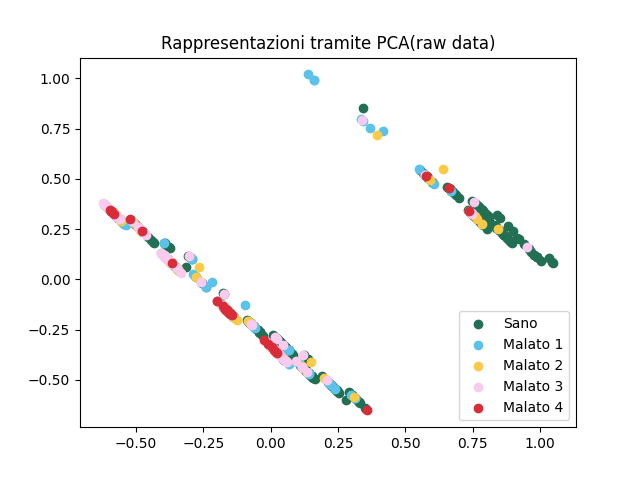
\includegraphics[width=0.5\linewidth]{imgs/pca.png}
        \label{fig:pca_data_visualization}
        \caption{Data visualization con PCA}
    \end{figure}
    PCA è un metodo \textbf{non supervisionato} per effettuare riduzione dimensionale dei dati.
    Questa funzione è molto utile per permettere la rappresentazione di dati multidimensionali
    in uno spazio bidimensionale scegliendo i dati con maggior varianza.

    
    \subsection{LDA}

    \begin{figure}[h!]
        \centering
            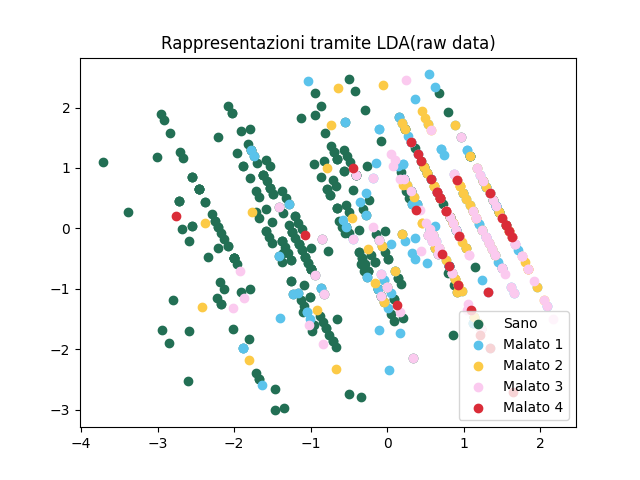
\includegraphics[width=0.5\linewidth]{imgs/lda.png}
        \label{fig:lda_data_visualization}
        \caption{Data visualization con LDA}
    \end{figure}

    LDA è un metodo \textbf{supervisionato} per effettuare riduzione dimensionale dei dati.

    Per effettuare la riduzione, crea un subset di features che rappresentano meglio la label target.

\subsection{Considerazioni PCA e LDA}

    Entrambi i grafici fanno riflettere sul fatto che non siano corretti.
    LDA per esempio, presenta una strana separazione in 4 classi. 

    \clearpage

    \subsection{Correlazioni tra i dati}

    \begin{figure}[h!]
        \centering
        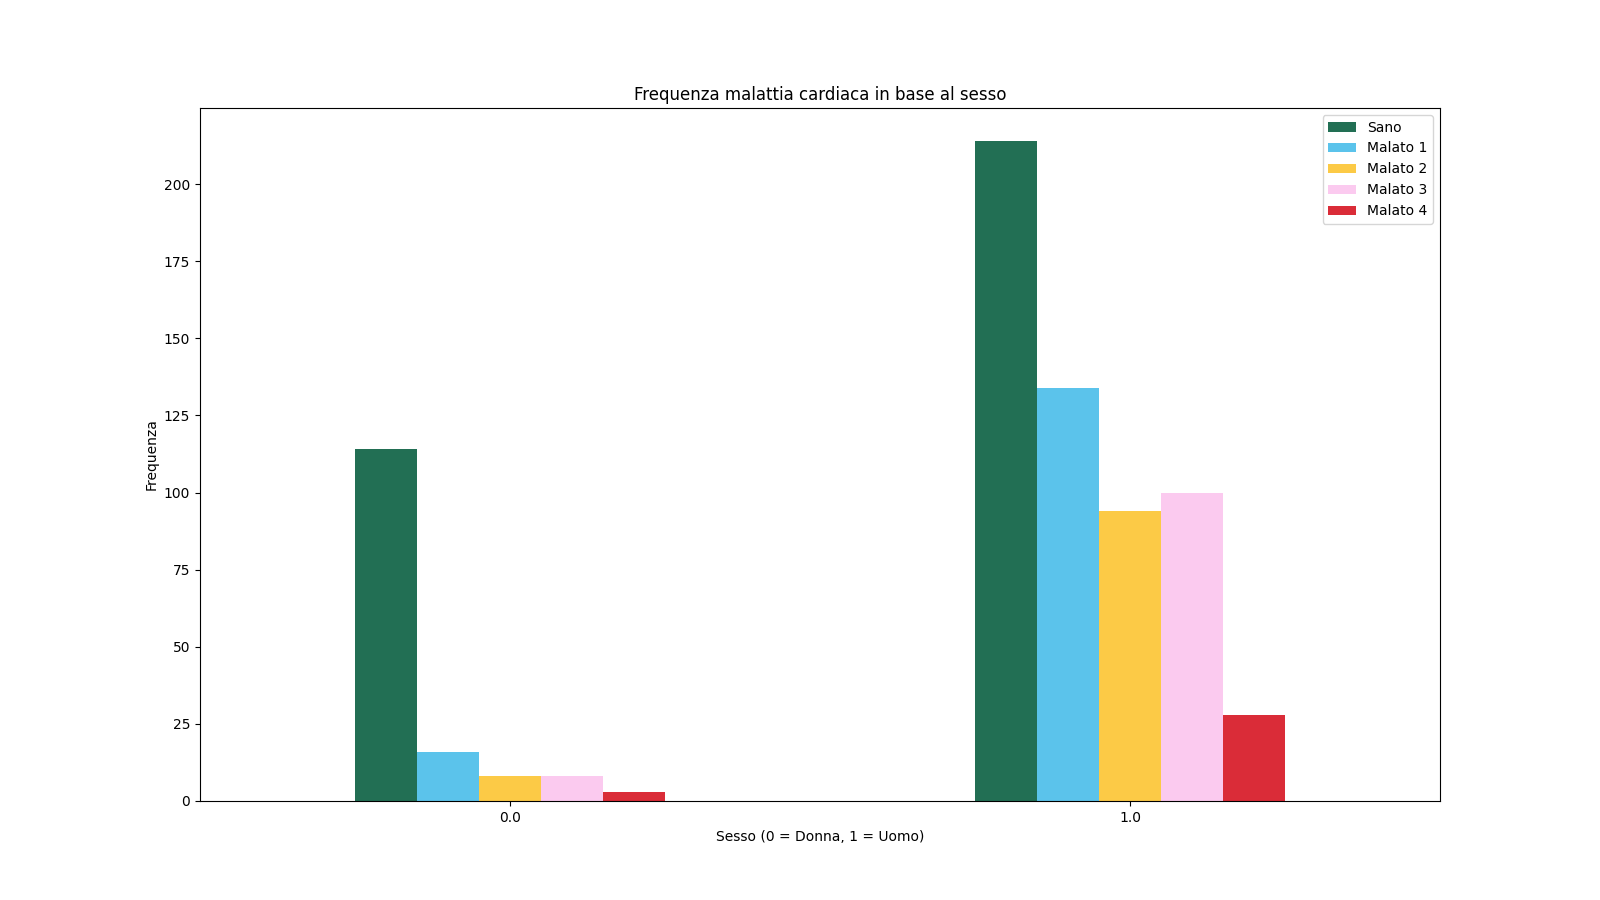
\includegraphics[width=0.5\linewidth]{imgs/sesso.png}
        \label{fig:sesso}
        \caption{Correlazione salute-sesso}
    \end{figure}

    Da questo grafico si possono dedurre due considerazioni:
    \begin{itemize}
        \item Maggioranza di persone di sesso maschile prese in considerazione per l'analisi
        \item Maggior probabilità di malattia cardiaca per gli uomini
    \end{itemize}

    \begin{figure}[h!]
        \centering
        \includegraphics[width=0.5\linewidth]{imgs/città.png}
        \label{fig:citta}
        \caption{Correlazione salute-città}
    \end{figure}
    
    Da questo grafico si può capire il motivo per la realizzazione di un'unico dataset.
    Come rappresentato nel grafico, si hanno pochissime istanze in long beach e switzerland,
    la capacità di apprendere correttamente dal dataset ne risente nelle classi meno rappresentate.

    \begin{figure}[h!]
        \centering
        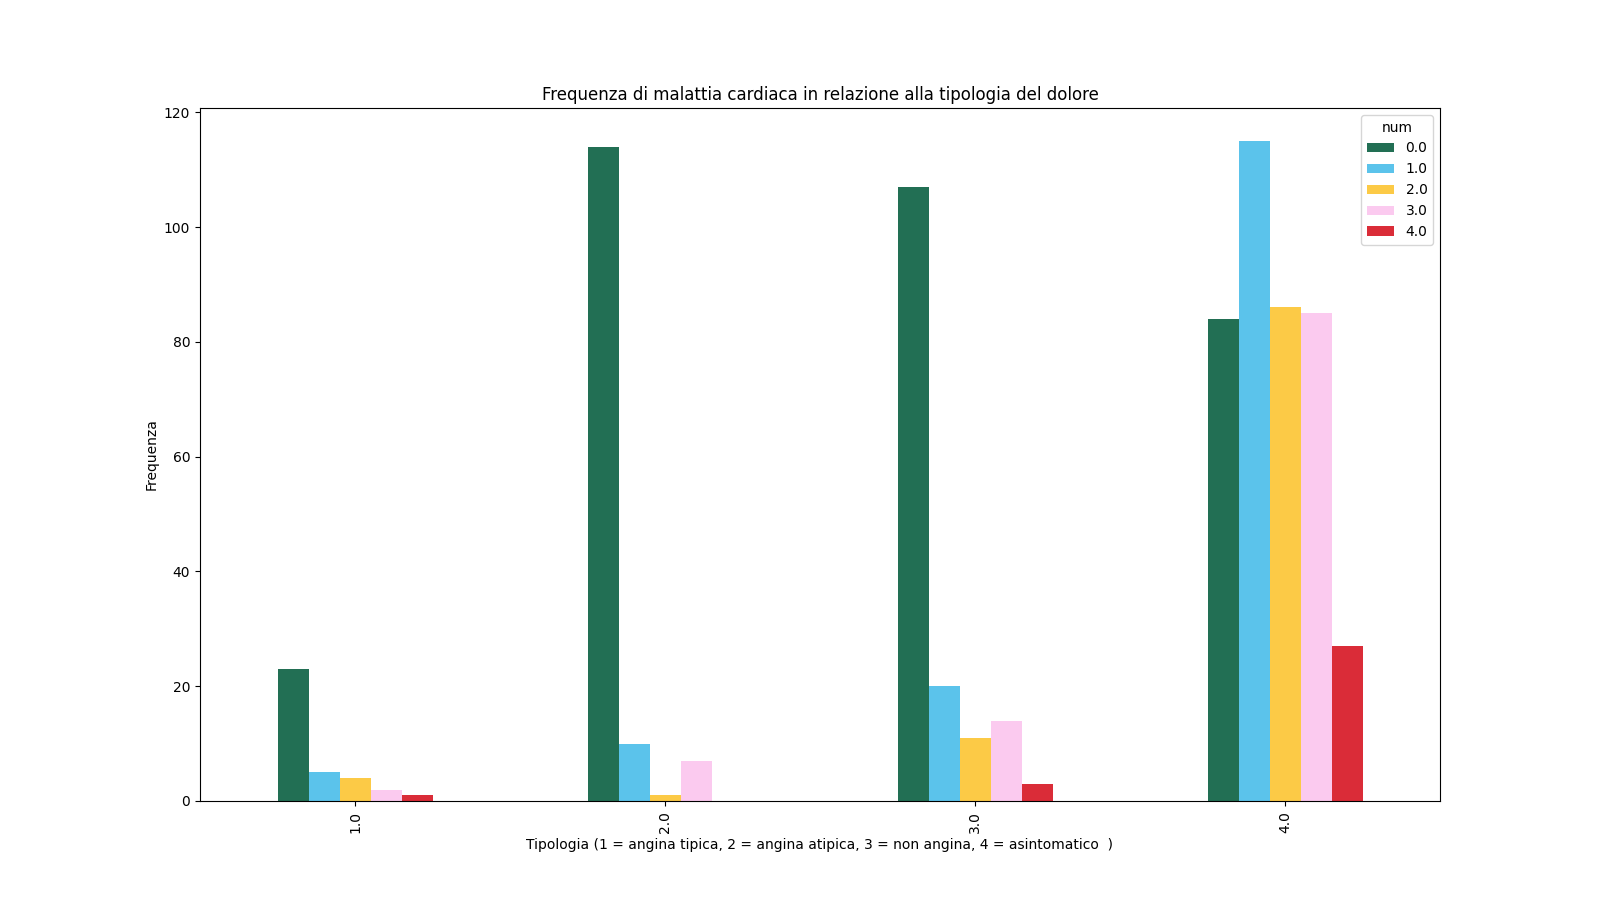
\includegraphics[width=0.5\linewidth]{imgs/tipologia dolore.png}
        \label{fig:dolore}
        \caption{Correlazione salute-dolore}
    \end{figure}

    Mediante questo grafico possiamo intuire che la maggior parte dei pazienti malati non presenti sintomi
    fisici(dolore al petto) nella quotidianità.


    \pagebreak
    \begin{figure}[h!]
        \centering
        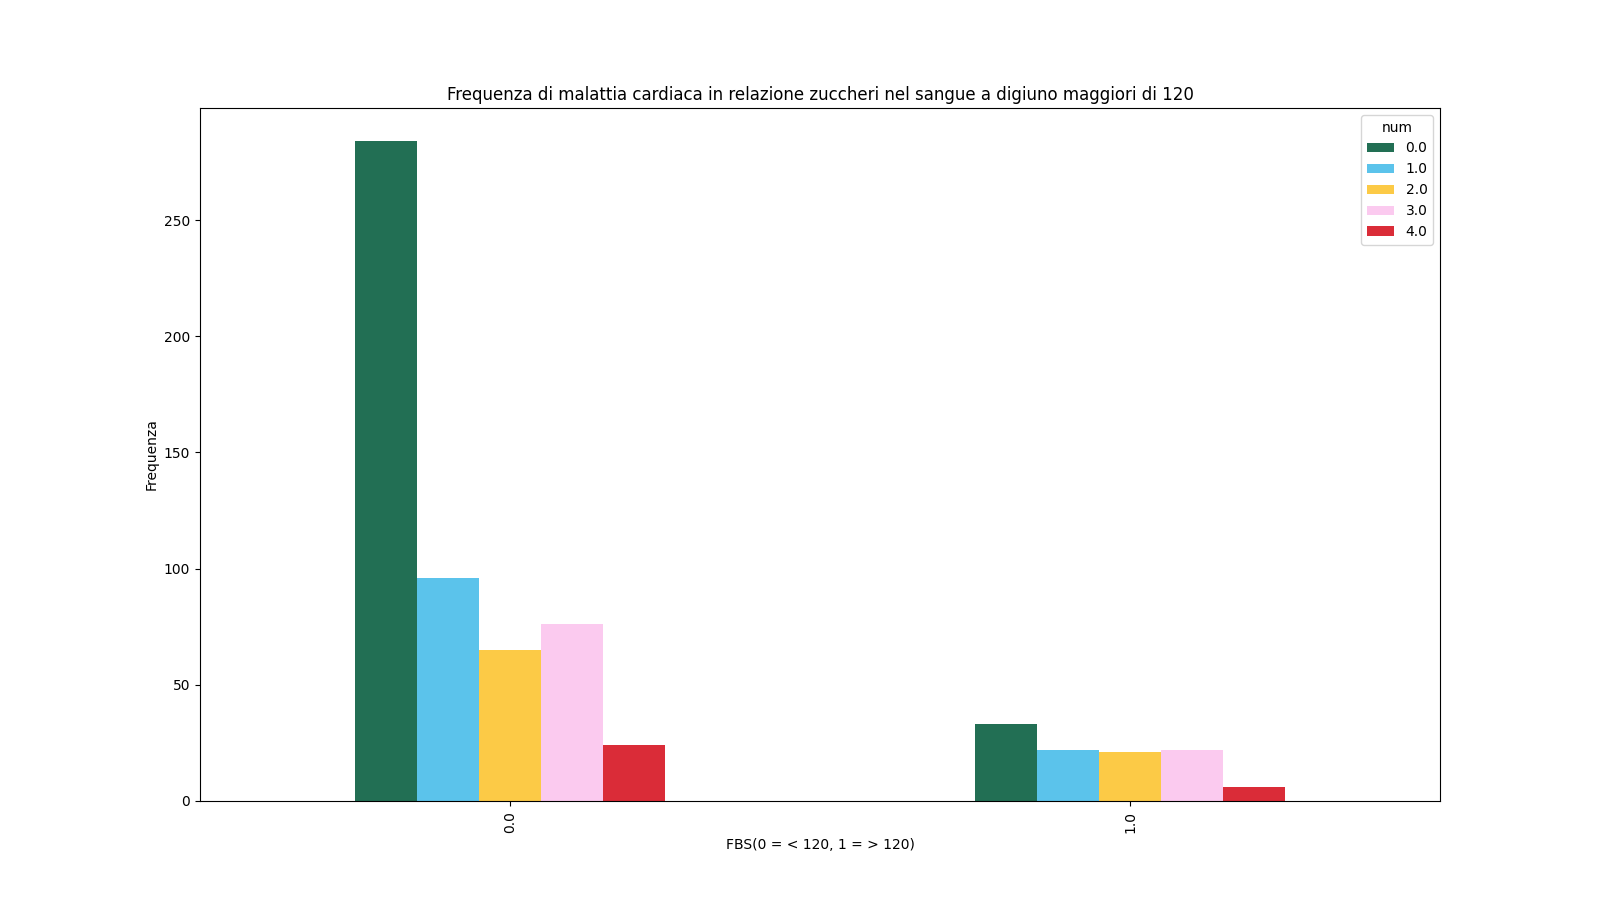
\includegraphics[width=0.5\linewidth]{imgs/zuccheri.png}
        \label{fig:zuccheri}
        \caption{Correlazione salute-zuccheri}
    \end{figure}

    Solitamente con una densità di zuccheri a digiuno superiore a $120mg/dL$ si viene considerati diabetici.
    Da questo grafico si può intuire che la percentuale di persone sottoposta all'analisi dei dati è prevalenetemente \textbf{non diabetica}.
    Qualora il paziente venga identificato come diabetico la probabilità di malattia cardiaca aumenta
    più del doppio rispetto ad un paziente non affetto dalla stessa.


    \begin{figure}[h!]
        \centering
        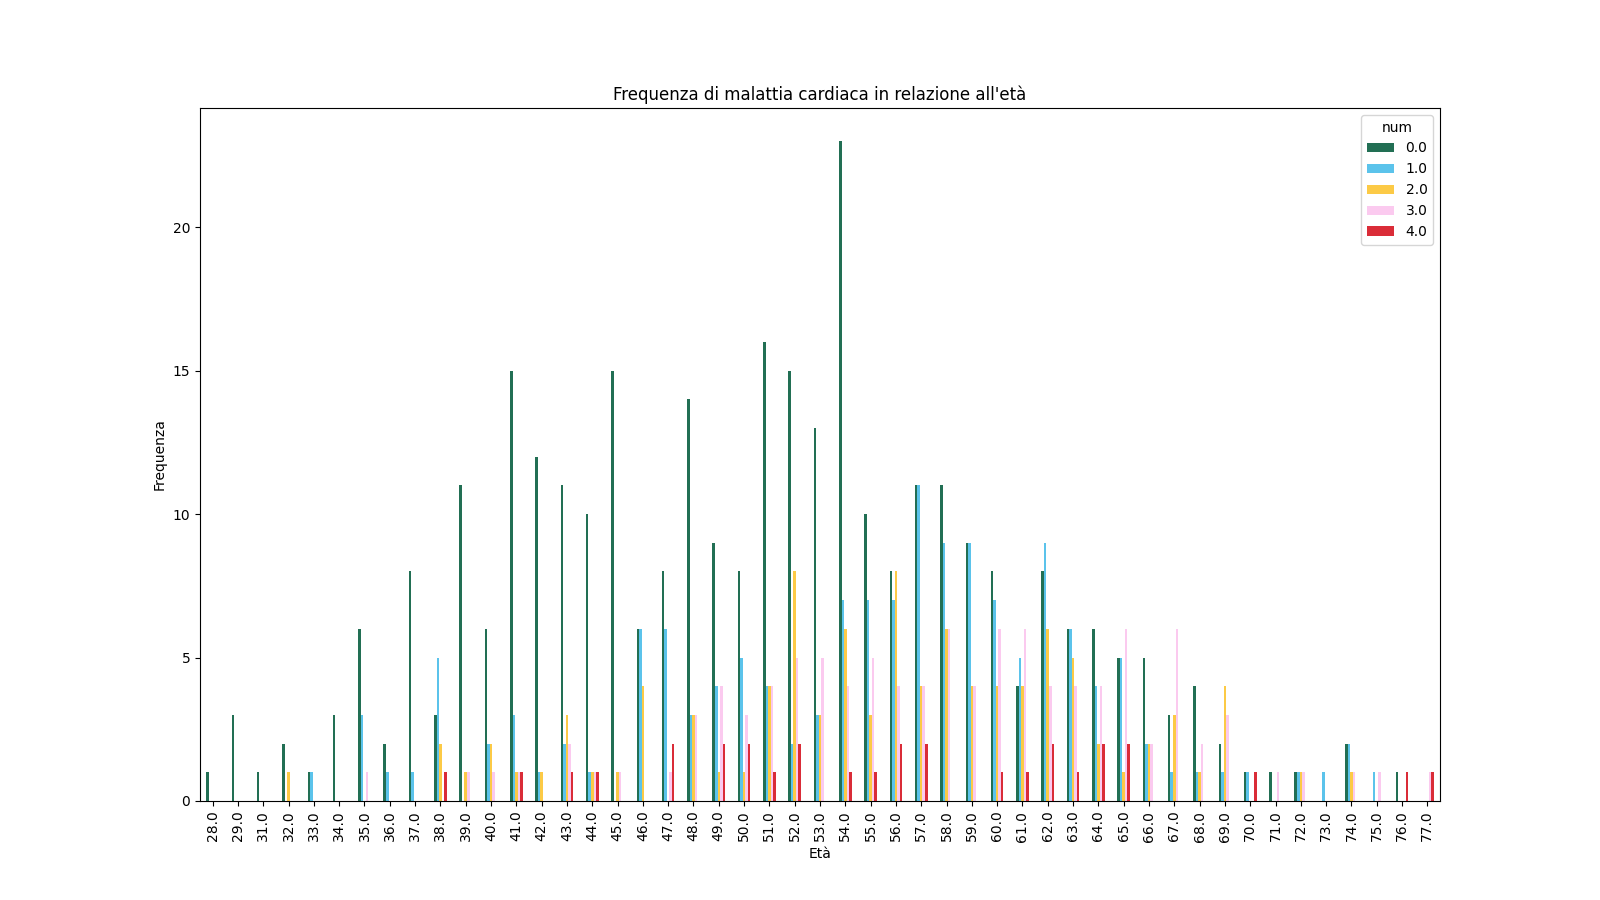
\includegraphics[width=0.9\linewidth]{imgs/età.png}
        \label{fig:eta}
        \caption{Correlazione salute-età}
    \end{figure}
    Con questo grafico si può visualizzare una distribuzione a campana dei pazienti in correlazione all'età.

    \section{Prepare data for ML algorithms}

    Questa è la parte più corposa del progetto poichè, in termini di codice, il dataset originale presenta 76 features di cui 1 classe target.


    \subsection{Non unique}
    In questa fase si sono cercate quelle features che non apportano informazioni, poichè costanti.

    È stata rimossa la features \textbf{PNCADEN}.

    \subsection{Analisi dei valori nulli}
    Nel dataset i valori nulli sono salavati con il valore di \textbf{$-9$}.
    Quindi il primo passo è stato quello di sostituire i valori con \textbf{pd.nan} che restituisce il valore nullo.

    Dopo aver ottenuto il dataset con i valori nulli, si è proseguito con il rimuovere tutte le colonne e tutte le righe
    contenenti una percentuale di valori nulli maggire del $15\%$.

    \subsection{Outliners}
    Per poter effettuare il processo di eliminazione degli outliners bisogna, per prima cosa, salvare i dati numerici in un
    array e successivamente analizzare la deviazione standard per includere solo il $99\%$ dei dati.

    Mediante la funzione \textbf{zscore} della libreria stats si sono eliminati gli esempi con una deviazione maggiore del 3.

    \subsection{Date}
    Studiando il problema si è pensato che le date non apportassero informazioni utili e si è preferito rimuoverle.
    

    \subsection{Variabile ``proto''}
    La variabile proto è una features categorica con 12 casistiche e rappresenta la tipologia del protocollo utilizzato 
    per il test da sforzo.

    Dal'analisi di questa features si è notato che la maggior parte dei valori non sono coerenti con le 12 classi.
    Si è di conseguenza preferito rimuovere l'intera colonna della feature.
    

    \subsection{Fillna}
    Si è provveduto ad assegnare la tipolgia ai dati(float, category, ecc) e successivamente assegnare, ai dati ancora nulli il valore medio
    presente per la propria colonna nel dataset.

    \subsection{Features selection}
    Dato che alcune features presentano valori negativi non si è potuto ricorrere al chi2 per l'analisi delle migliori features.
    
    Si è scelto di utilizzare due funzioni:
    \begin{itemize}
        \item ANOVA con la funione f classif
        \item mutaul info regression
    \end{itemize}


    Mutual info regression ha attribuito il risultato più basso alle seguenti features:
    \begin{itemize}
        \item xhypo
        \item htn
        \item diuretic
        \item trestbpd
        \item thalrest
        \item nitr
        \item tpeakbps
        \item prop
        \item pro
    \end{itemize}


    Anova ha attributo il risultato più basso alle seguenti features:
    \begin{itemize}
        \item tpeakbpd
        \item dig
    \end{itemize}

    Il risultato finale dopo il datacleaning è il seguente sub-set:
    \begin{center}
        \scalebox{0.7}{
            \def\arraystretch{1.5}
        \begin{tabular}{| p{20mm} | p{50mm} |}
            \hline
            Nome & Descrizione \\
            \hline
            age & Età del soggetto \\
            sex & Sesso del soggetto(0 = F, 1 = M) \\
            cp & Tipologia di dolore al petto \\
            trestbps & Pressione a riposo \\
            chol & colesterolo \\
            fbs & zuccheri nel sangue a digiuno maggiori di $120mg/dl$, 1 = vero, 0 = falso \\
            restecg & Elettrocardiogramma a riposo, 0 = normale, 1 = anormale \\
            thaldur & durata esercizio in minuti \\
            met & metriche raggiunte \\
            thalach & Battiti masimi \\
            exang & Angina indotta dall'esercizio? 1 = si, 0 = no \\
            oldpeak & calo di pressione indotto a riposo \\
            location & variabile encodata per rappresentare il dataset di provenienza \\
            target & Rappresenta la classe che identifica la presenza e lo stato della malattia(usato come Y) \\
            \hline            
        \end{tabular}
        }
    \end{center}

    

    \section{Model comparison}
    Ad ogni modello è stato applicata una k-fold di 10 e sono state effettuate prove con il dataset ottenuto dalla features
    selection.
    Per lo stesso dataset sono state eseguite prove anche con un dataset bilanciato ottenuto tramite oversampling(smote).
    

    \begin{figure}[!h]
        \centering
        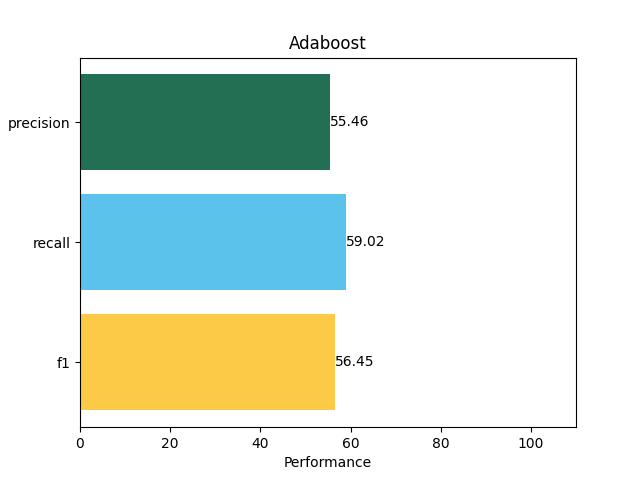
\includegraphics[width=0.4\linewidth]{scores/ada boost.png}
        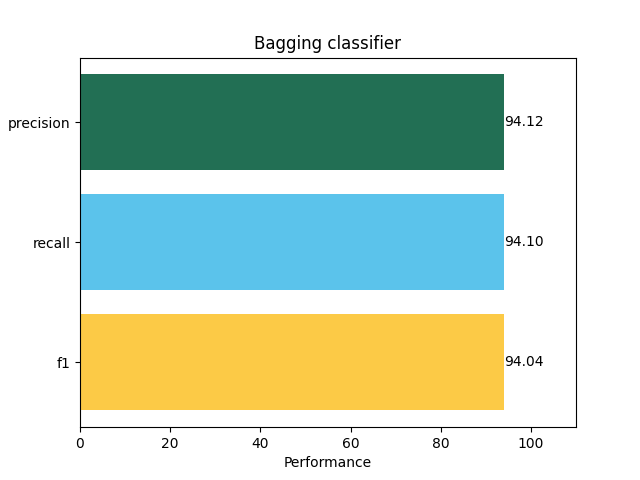
\includegraphics[width=0.4\linewidth]{scores/bagging classifier.png}
        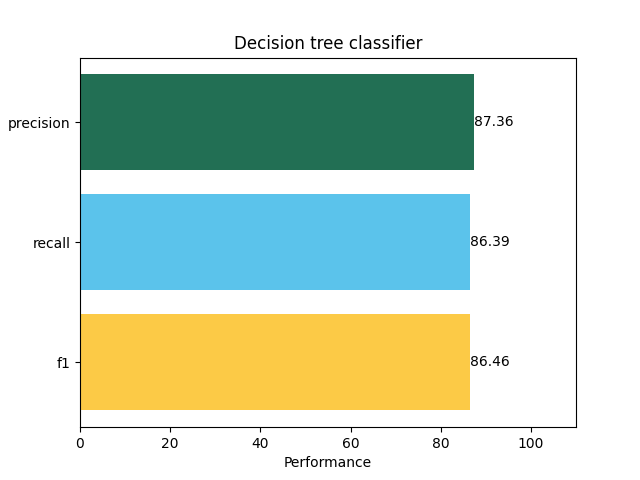
\includegraphics[width=0.4\linewidth]{scores/decision tree classifier.png}
        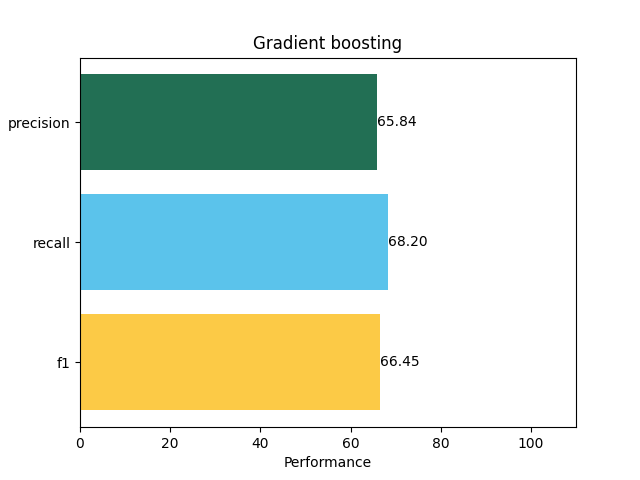
\includegraphics[width=0.4\linewidth]{scores/gradient boosting.png}
    \end{figure}

    \begin{figure}[!h]
        \centering
        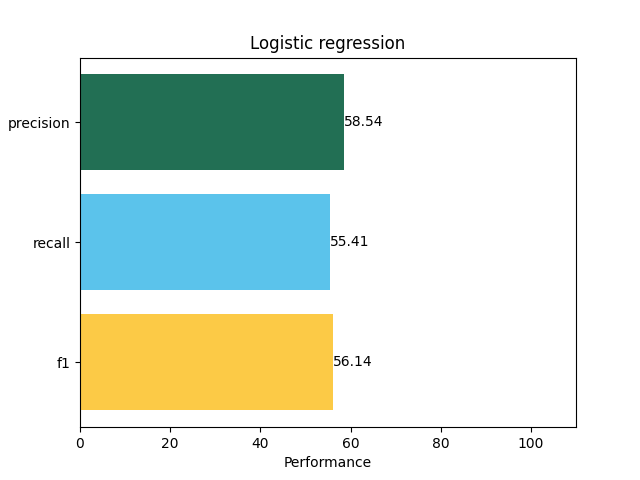
\includegraphics[width=0.4\linewidth]{scores/logistic regression.png}
        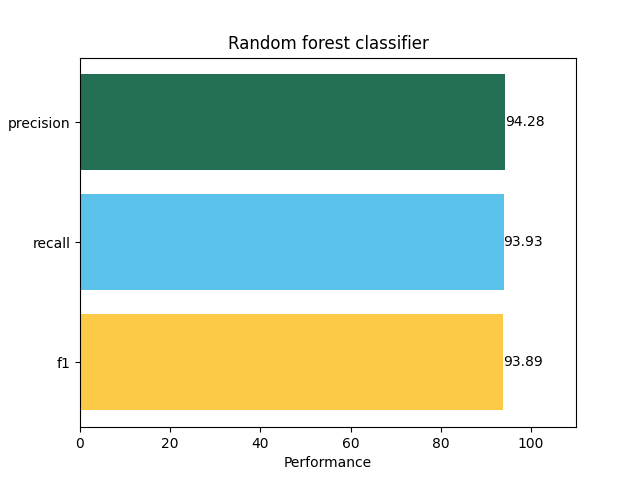
\includegraphics[width=0.4\linewidth]{scores/random forest classifier.png}
        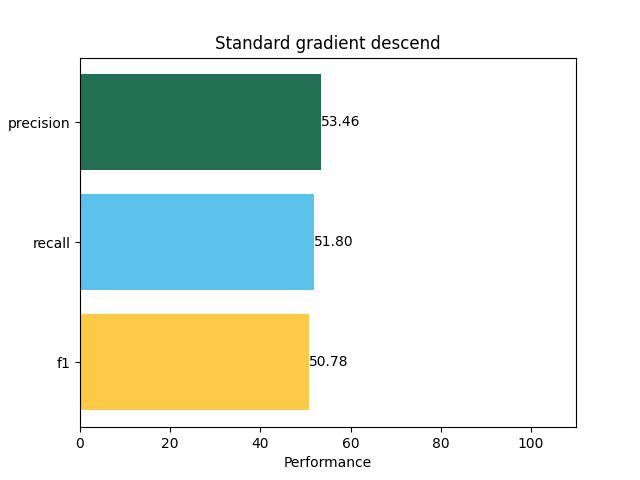
\includegraphics[width=0.4\linewidth]{scores/standard gradient descend.png}
        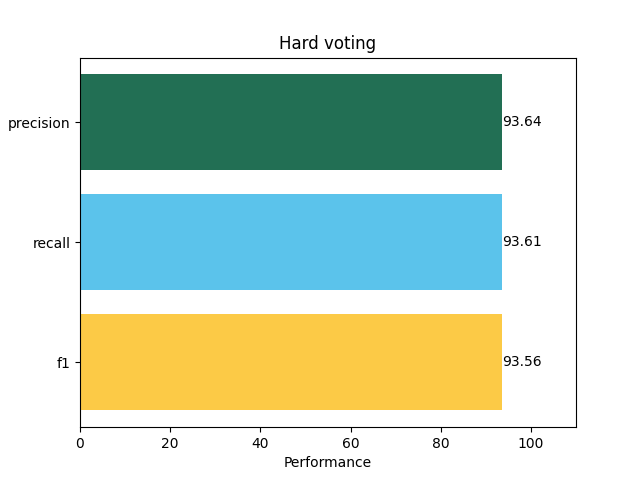
\includegraphics[width=0.4\linewidth]{scores/hard voting.png}

    \end{figure}

    Dopo un controllo con il train-set iniziale si è capito che smote non migliora i punteggi e di conseguenza
     si è preferito mantenere il dataset sbilanciato.

    \section{Evaluation}

    Ogni modello è stato ``fittato'' 10 volte mediante k-fold sia con dati sbilanciati che con dati bilanciati tramite 
    over sampling.
    
    Sono stati regolati i parametri di fine tuning e, una volta ottenuto il risultato migliore,
    si è provveduto a fare la prova finale con il test-set separato all'inizione del processo
    di machine learning.

    Considerata la natura del test, cioè dover prevedere se un paziente sia malato o meno, si è preferito dare
    leggermente maggior importanza al punteggio di \textbf{recall}, essendo il recall il valore che rappresenta
    la misura dell'errore sui ``false positive''.
    
    Pertanto i modelli migliori che risultano da questa analisi sono:
    \begin{itemize}
        \item Bagging classifier
        \begin{itemize}
            \item precision $= 94.12\%$
            \item recall $= 94.10\%$
            \item f-1 $= 94.04\%$
        \end{itemize}
        \item Random forest classifier
        \begin{itemize}
            \item precision $= 94.28\%$
            \item recall $= 93.93\%$
            \item f-1 $= 93.89\%$
        \end{itemize}
        \item Hard voting
        \begin{itemize}
            \item precision $= 93.64\%$
            \item recall $= 93.61\%$
            \item f-1 $= 93.56\%$
        \end{itemize}
    \end{itemize}

    \section{Fonti}
    Il dataset proviene da: UCI machine learning repository.

    Creatori:
    \begin{itemize}
        \item Hungarian Institute of Cardiology. Budapest: Andras Janosi, M.D. 
        \item University Hospital, Zurich, Switzerland: William Steinbrunn, M.D.
        \item University Hospital, Basel, Switzerland: Matthias Pfisterer, M.D. 
        \item V.A. Medical Center, Long Beach and Cleveland Clinic Foundation: Robert Detrano, M.D., Ph.D.
    \end{itemize}
    Donatore:
    \begin{itemize}
        \item David W. Aha (aha '@' ics.uci.edu)
    \end{itemize}
\end{document}